% !TEX TS-program = pdflatex
% !TEX encoding = UTF-8 Unicode

% This is a simple template for a LaTeX document using the "article" class.
% See "book", "report", "letter" for other types of document.

\documentclass[11pt]{article} % use larger type; default would be 10pt

\usepackage[utf8]{inputenc} % set input encoding (not needed with XeLaTeX)

%%% Examples of Article customizations
% These packages are optional, depending whether you want the features they provide.
% See the LaTeX Companion or other references for full information.

%%% PAGE DIMENSIONS
\usepackage{geometry} % to change the page dimensions
\geometry{a4paper} % or letterpaper (US) or a5paper or....
% \geometry{margin=2in} % for example, change the margins to 2 inches all round
% \geometry{landscape} % set up the page for landscape
%   read geometry.pdf for detailed page layout information

\usepackage{graphicx} % support the \includegraphics command and options

% \usepackage[parfill]{parskip} % Activate to begin paragraphs with an empty line rather than an indent

%%% PACKAGES
\usepackage{booktabs} % for much better looking tables
\usepackage{array} % for better arrays (eg matrices) in maths
\usepackage{paralist} % very flexible & customisable lists (eg. enumerate/itemize, etc.)
\usepackage{verbatim} % adds environment for commenting out blocks of text & for better verbatim
\usepackage{subfig} % make it possible to include more than one captioned figure/table in a single float
% These packages are all incorporated in the memoir class to one degree or another...

\usepackage{hyperref}
\usepackage{amsmath, amssymb, amsthm}
\newtheorem{theoreme}{Theoreme}[section]
\newtheorem{definition}{Définition}[section]
\newtheorem{proposition}{Proposition}[section]
\newtheorem{corollary}{Corollary}[section]
\newtheorem{conjecture}{Conjecture}[section]
\usepackage{bbm}
%%% HEADERS & FOOTERS
\usepackage{fancyhdr} % This should be set AFTER setting up the page geometry
\pagestyle{fancy} % options: empty , plain , fancy
\renewcommand{\headrulewidth}{0pt} % customise the layout...
\lhead{}\chead{}\rhead{}
\lfoot{}\cfoot{\thepage}\rfoot{}

%%% SECTION TITLE APPEARANCE
\usepackage{sectsty}
\allsectionsfont{\sffamily\mdseries\upshape} % (See the fntguide.pdf for font help)
% (This matches ConTeXt defaults)

%%% ToC (table of contents) APPEARANCE
\usepackage[nottoc,notlof,notlot]{tocbibind} % Put the bibliography in the ToC
\usepackage[titles,subfigure]{tocloft} % Alter the style of the Table of Contents
\renewcommand{\cftsecfont}{\rmfamily\mdseries\upshape}
\renewcommand{\cftsecpagefont}{\rmfamily\mdseries\upshape} % No bold!

%%% END Article customizations

%%% The "real" document content comes below...

\title{Note décomposition en ondelettes complexes}
\author{Leo Davy}
%\date{} % Activate to display a given date or no date (if empty),
         % otherwise the current date is printed 

\begin{document}
\maketitle
\section{Ondelettes complexes et Dual Tree Complex Wavelet Transform}
\subsection{Modèle standard}
On se donne une base d'ondelettes $(\psi_{j,k})$ et on considère les coefficients d'ondelettes
\begin{equation}
	d_j(x) = \langle X, \psi_{j,k_x} \rangle = X\star \psi_j (x)
\end{equation}
d'un signal $x\mapsto X(x)$. Afin de gagner en invariance par translation (locale) (?) on s'intéresse plutôt aux (log-)leaders en prenant au lieu de $d_j(x)$ le supremum des valeurs absolues des coefficients de tous les coefficients dans le voisinage de $k_x$ à toutes les échelles les plus fines. Pour alléger les notations, je confonds les notations pour les coefficients d'ondelettes et les leaders. On a ainsi
\begin{equation}
	d_j(x) \sim v(x)2^{jh(x)}\xi_x=^\mathbb{E} v(x)2^{jh(x)}
\end{equation}
avec $\xi_x$ un bruit multiplicatif, centré en 1, log-normal si on veut un bruit gaussien sur les logs-leaders, qu'on ignore par la suite et on considère les égalités en espérance. En passant au log on est ramené à une régression linéaire. Par contre, l'analyse est isotrope parce que au début de l'analyse en dimension $d$, on a $2^d - 1$ ondelettes $\psi$, vu que par hypothèse le signal est isotrope, et localement homogène, afin de diminuer l'impact du bruit $\xi$, on considère chaque coefficient d'ondelette de façon uniforme (par rapport aux directions). On n'a donc pas d'espoir de récupérer des informations spécifiques aux directions. 

\subsection{Modèle complexe}
A la place d'une ondelette réelle, on peut considérer une ondelette complexe pour faire l'analyse, de la forme :
\begin{equation}\label{eq:ondeletteC}
	\psi = Re(\psi) + iIm(\psi) = \psi_r + i\psi_c
\end{equation}
où $\psi_r$ et $\psi_c$ sont des ondelettes réelles. 
En particulier, elles peuvent vérifier
\begin{equation}\label{eq:modele}
	d_j^{r,c}(x) = v_{r,c}(x)2^{jh_{r,c}(x)}
\end{equation}
où l'équation est à considérer soit pour $r$, soit pour $c$ (par exemple, $h_r$ désigne la régularité au sens de la quantité de multirésolution associée à l'analyse par l'ondelette réelle $\psi_r$). On se retrouve donc avec des coefficients complexes d'ondelette
\begin{equation}
	d_j(x) = d_j^r(x) + id_j^c(x) = v_r(x)2^{jh_r(x)} + iv_c(x)2^{jh_c(x)}.
\end{equation}
On peut alors réécrire l'expression précédente, en ignorant la dépendance en $x$, sous la forme
\begin{equation}\label{eq:leadlead}
	d_j = \sqrt{v_r^22^{2jh_r} + v_c^22^{2jh_c} } e^{i \arctan{\left(\frac{v_c2^{jh_c}}{v_r2^{jh_r}} \right)} } = \rho_je^{i\omega_j}
\end{equation}
avec
\begin{equation}
	\rho_j(x) := \sqrt{v_r(x)^22^{2jh_r(x)} + v_c(x)^22^{2jh_c(x)} }
\end{equation}
et 
\begin{equation}
	\omega_j(x) = \arctan{\left(\frac{v_c(x)}{v_r(x)}2^{j(h_c(x) - h_r(x))} \right)}.
\end{equation}
Que l'on peut aussi réécrire sous la forme
\begin{equation}
	d_j(x) = \rho_j(x) \cos(\omega_j(x)) + i\rho_j(x)\sin(\omega_j(x)).
\end{equation}
En particulier, on peut remarquer 
\begin{enumerate}
	\item que le module ($\rho_j$) et la phase ($\omega_j$) de $d_j$ sont indépendants (l'expression de l'une des deux quantités ne fait pas intervenir l'autre).
	\item $\log(\tan(\omega_j)) =\log(d_j^c/d_j^r)$ permet une régression linéaire de $\log{\frac{v_c}{v_r}}$ et $h_c - h_r$.
	\item Comme $d_j$ provient d'une analyse en ondelettes, on peut peut être aussi supposer que $\rho_j \sim v2^{jh}$ et estimer $\log(v)$ et $h$ aussi par régression linéaire de $\log(\rho_j)$
	\item Aussi, il y a sûrement un lien entre les deux quantités précédentes qui pourrait permettre de coupler les estimations.
\end{enumerate}
\par
On peut donner une intuition au fait que $\omega$ mesure bien un angle dans la texture de la manière suivante. On suppose $v_c/v_r$ constant et donc $\omega_j$ ne dépend que de $2^{j(h_c - h_r)}$. Dans un premier temps on suppose $h_c >>h_r$, c'est à dire que la quantité multirésolution associée à l'ondelette $\psi_c$ décroit plus vite que celle associée à $\psi_r$; ou bien, plus simplement, $X$ est plus régulier suivant l'ondelette $c$ que l'ondelette $r$. 
\newline
Donc quand on considère les échelles les plus fines ($j\to -\infty$) on a $\omega_j \to \arctan(0)$, d'où, aux échelles les plus fines, la phase disparait et toute l'information est capturée par l'ondelette $\psi_r$. Cela correspond probablement à ce qu'on attend, car $h_c > h_r$ signifie qu'il y a plus d'information locale suivant $\psi_r$ que $\psi_c$.
\newline
En considérant $h_c<<h_r$ on peut appliquer le même raisonnement et obtenir que l'information est capturée seulement par l'ondelette $h_c$.
\par
Il reste donc à s'assurer que $\psi_r$ et $\psi_c$ capturent bien de l'information dans des directions distinctes. Pour cela, la stratégie semble être de choisir des ondelettes $\psi_r$ et $\psi_c$ qui sont obtenues par transformée de Fourier d'ondelettes $\phi_r$ et $\phi_c$.
C'est à dire, par exemple,
\begin{equation}
	\psi_r(t) = \hat{\phi_r}(t).
\end{equation}
Et ainsi, un signal anisotrope $X(t)$ qui a une densité spectrale de la forme $|\hat{X}(\zeta)| \leq \frac{1}{||\zeta||^{h(\zeta)}}$, où $\zeta \mapsto h(\zeta)$ est une fonction qui ne dépend que de l'angle, qui donne la régularité directionnelle (pour des directions spectrales).
\par
Donc, si, par exemple si $\Omega$ est le support de $\phi_r$, on a
\begin{equation}
	d_{j=0}^r = \langle X, \psi_r \rangle = \langle X, \hat{\phi_r}\rangle = \langle \hat{X}, \phi_r \rangle
\end{equation}
et donc $d_0^r$ ne dépend que des directions (en Fourier) de $X$ supportées dans $\Omega$. Il reste à voir quelles propriétés on souhaite avoir entre $\psi_r$ et $\psi_c$. On pourra par exemple chercher à avoir que $\rho_j$ soit une quantité anisotrope, au sens où si $X^\theta$ est une rotation par $\theta$ d'un signal $X$, alors leur coefficients complexes d'ondelettes ont même module. Cela forcerait l'information sur l'anisotropie à être contenue dans $\omega_j$ (peut-être que c'est trop restrictif et que l'on perdrait toute l'information sur l'anisotropie).

\subsubsection{Une version plus précise}
	Ci-dessus tout a été noté avec des coefficients d'ondelettes $d_{j,k}(X) = \langle X,\psi_{j,k}\rangle$, qui ne vérifient pas en général le modèle \ref{eq:modele} contrairement aux leaders
\begin{equation}
	l_{j,k} = \sup_{\lambda_{j',k'}\subset 3\lambda_{j,k}} 2^{j-j'}|d_{j',k'}|
\end{equation}
où les $\lambda_{j,k}$ sont des cubes $[2^jk, 2^j(k+1))$ pour des signaux en une dimension (et la multiplication se fait par homotéthie). En dimension $d$,
\begin{equation}
	l_{j,k} : = l^{p=\infty}(j,k) = \left( \sum_{\lambda_{j',k'}\subset 3\lambda_{j,k} } 2^{-d(j-j') }||d_{j,k}||_{\ell^{p=\infty}(2^d-1)} \right) = \sup_{\lambda_{j', k'}\subset 3\lambda_{j,k}} \sup_i 2^{d(j-j')}| d^{(i)}_{j',k'}|
\end{equation}
où on passe par la définition des $p$-leaders et $d_{j,k} =(d_{j,k}^{(i=1)},\cdots, d_{j,k}^{(i=2^d-1)})$ sont les coefficients d'ondelettes en dimension $d$.
\newline
Un problème qui apparait peut être avec cette définition est que l'on perd complétement l'information sur l'ondelette dont provient le leader choisi, alors que chaque ondelette $i$ peut avoir des propriétés directionnelles particulières. Une solution est peut-être de considérer des leaders pour chaque $i$ (mais l'un des problèmes est que l'on a un nombre de leaders exponentiel avec la dimension) :
\begin{equation}
	l_{j,k}^{(i)} = \sup_{\lambda_{j',k'}\subset 3\lambda_{j,k}} 2^{d(j-j')}|d_{j',k'}^{(i)}|.
\end{equation}
\subsection{Choix des ondelettes complexes}
	On s'intéresse maintenant au choix des ondelettes complexes sous la forme \ref{eq:ondeletteC}:
\begin{equation}
	\psi = \psi_r + i\psi_c.
\end{equation}
Les premières relations que l'on souhaite vérifier sont les relations d'échelles (écrites correctement avec les leaders cette fois-ci):
\begin{equation}
	l^{r,c}_{j,k} = \sup_{\lambda_{j',k'} \subset 3\lambda_{j,k}} 2^{d(j-j')}|d_{j',k'}^{r,c}| \sim v_{j,k}2^{jh_{j,k}^{r,c}}
\end{equation}
ainsi que 
\begin{equation}\label{eq:leadcoef}
	l_{j,k} = \sup_{\lambda_{j',k'}\subset 3\lambda_{j,k}} 2^{d(j-j')}|\langle X, \psi_{j',k'}\rangle| = \sup2^{d(j-j')}\sqrt{(d_{j',k'}^r)^2 + (d_{j',k'}^c)^2} \sim v_{j,k}2^{jh_{j,k}}
\end{equation}
qui sont vérifiées dès que $\psi_r$ et $\psi_c$ ont suffisament de moments nuls (et de régularité). 
\newline
On souhaite aussi faire une analyse locale, donc $\psi_r$ et $\psi_c$ doivent être \emph{localisées} (support compact).
\newline
Une autre propriété que l'on veut probablement est l'\emph{invariance par translation locale} pour autant de coefficients d'ondelettes que possible.
\newline
On peut aussi remarquer que les leaders complexes \ref{eq:leadcoef} "classiques" ne correspondent pas directement aux coefficients que l'on peut utiliser pour le modèle de régression écrit au début \ref{eq:leadlead}:
\begin{equation}
	\tilde l_{j,k} =|\sqrt{(l_{j,k}^r)^2 + (l_{j,k}^c)^2}e^{i\arctan\left(\frac{l_{j,k}^r}{l_{j,k}^c}\right)}|.
\end{equation}
Il serait appréciable que les deux quantités coincident.
\newline
Aussi, on s'intéresse à l'orientation, on voudrait donc que les ondelettes $\psi^{(i)}$ aient des propriétés directionnelles.
\newline
Une solution partielle à ces problèmes\footnote{cf réf sur Dual Tree Complex Wavelet, partie "Trouble in paradise : four problems with real wavelets"}, inspirés de la transformée de Fourier pour les signaux réels consiste à prendre 
\begin{equation}
	\psi = \psi_r + i\psi_c
\end{equation}
avec $\psi_r$ paire, et $\psi_i$ impaire, toutes deux réelles. De plus, si $\psi_r$ et $\psi_c$ sont déphasées de $\pi/2$ alors $\psi$ est un signal analytique. Par contre, dans ce cas là, $\psi$ ne peut pas être à support compact.
\subsection{Dual Tree Complex Wavelet Transform (DTCWT)}
Les DTCWT semblent être une option afin de contourner ce problème analyticité/support fini en utilisant une représentation (en ondelettes) redondante. L'idée est de choisir $\psi$ approximativement analytique, ou de façon équivalente, telle que $\psi_c$ soit approximativement la transformée de Hilbert de $\psi_r$.
\par
On utilise donc une paire d'ondelettes réelles, et on calcule la transformée en ondelettes pour chacune de ces ondelettes, l'une donne la partie réelle de l'ondelette complexe, et l'autre la partie imaginaire de l'ondelette complexe.
\newline
On peut calculer ces coefficients à partir de deux banques de filtres en parallèle, avec $r_0, r_1$ (resp $c_0, c_1$) les filtres passe-bas et passe-haut associés à l'ondelette réelle (resp. complexe).
\newline
Une condition simple pour avoir la propriété de quasi-analyticité dans le cas discret est que les filtres passe bas soient décalés d'un demi échantillon
\begin{equation}
	c_0(k) = r_0(k-0.5).
\end{equation}
Il semble donc que l'on cherche une paire de filtres à support fini vérifiant cette condition et dont les ondelettes associées ont suffisamment de moments nuls (et de régularité).
\newline
En dimension 2, on calcule 3 coefficients d'ondelette complexe par point, les parties réelles et imaginaires de chacun de ces coefficients est calculé à partir de deux ondelettes réelles séparables (mais aucune des six ondelettes n'est séparable), donc le calcul reste rapide.
Il est aussi possible d'augmenter la sensibilité par rapport à l'orientation, en utilisant la Real Oriented 2D Dual Tree Transform, qui donne 6 coefficients complexes par point.
\newline
Quelques références
\begin{enumerate}
	\item Sur Dual Tree Complex Wavelet Transform\url{https://ieeexplore.ieee.org/document/1550194}
\end{enumerate}
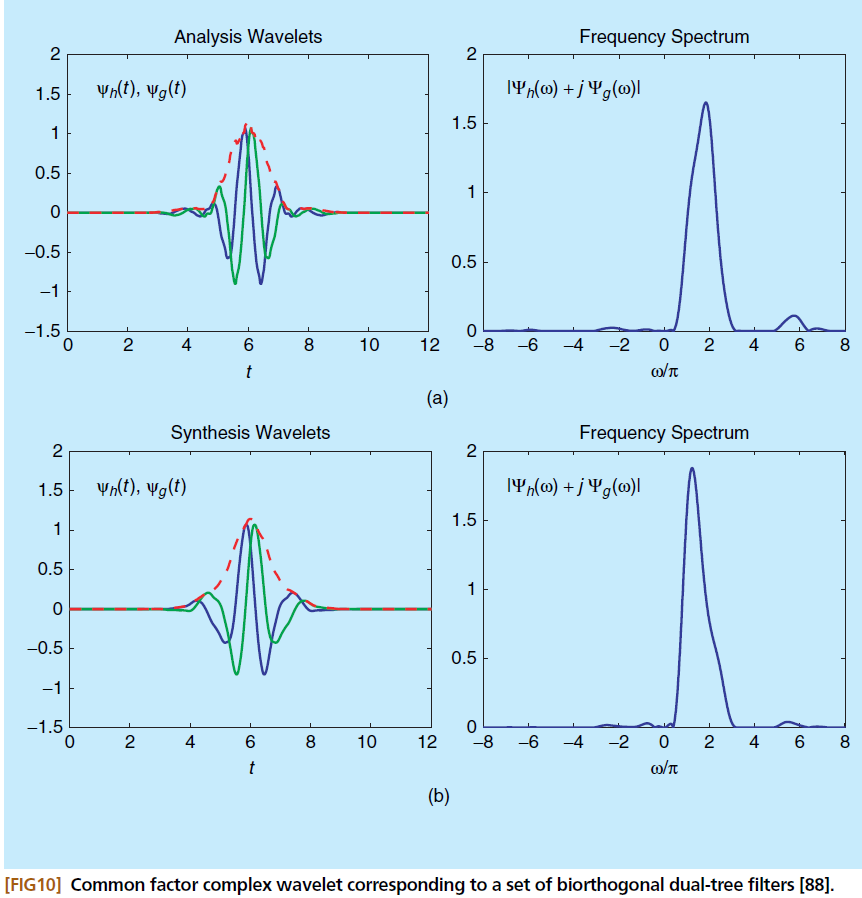
\includegraphics[width=0.6\textwidth]{dtcwt_wav}
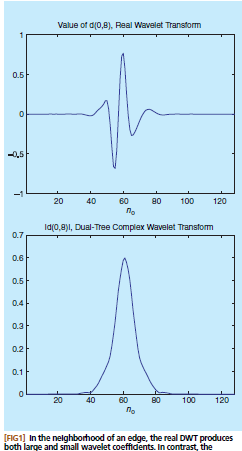
\includegraphics[width=0.3\textwidth]{realvscomplex}

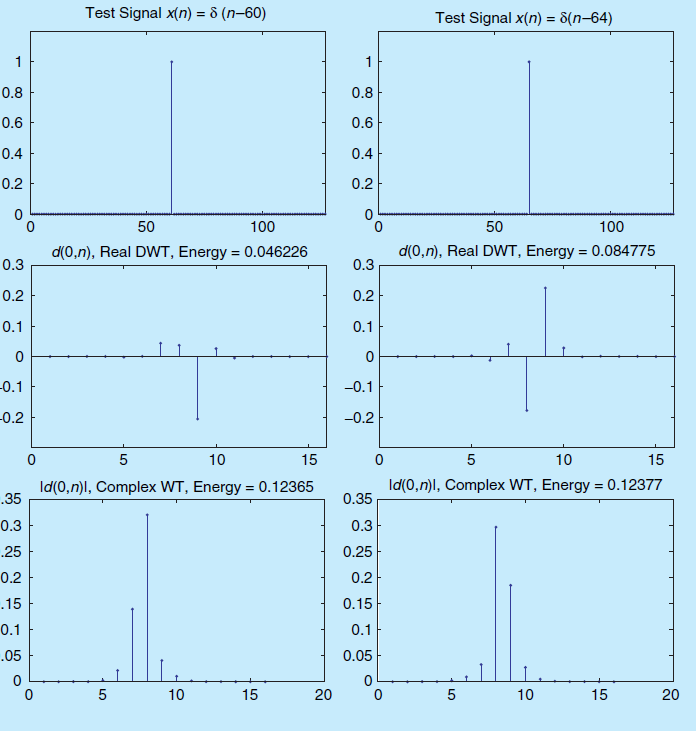
\includegraphics[width=0.9\textwidth]{coefstab}

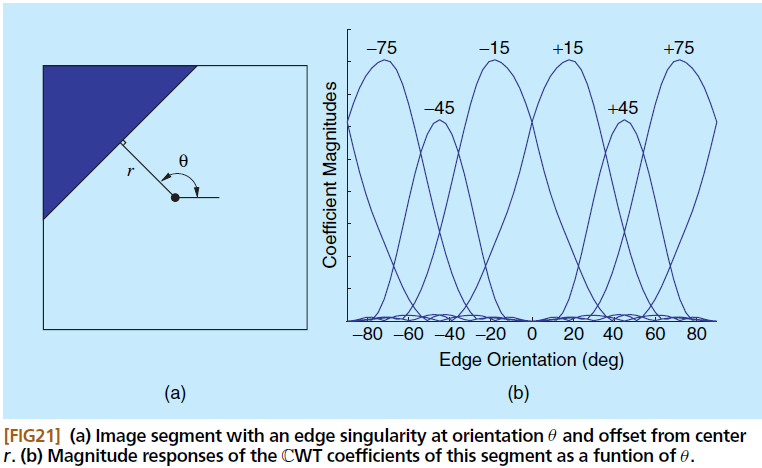
\includegraphics[width=\textwidth]{dt_edge}
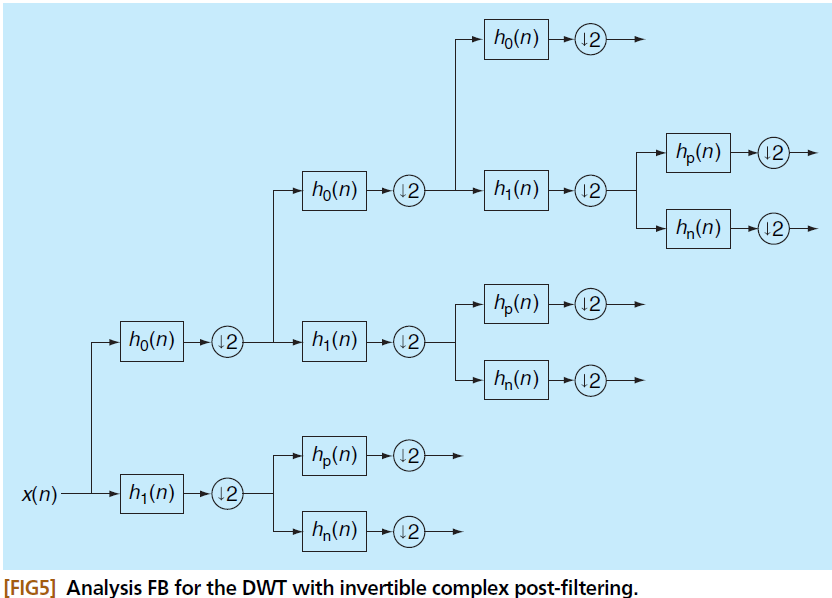
\includegraphics[width=\textwidth]{DWT_fb}
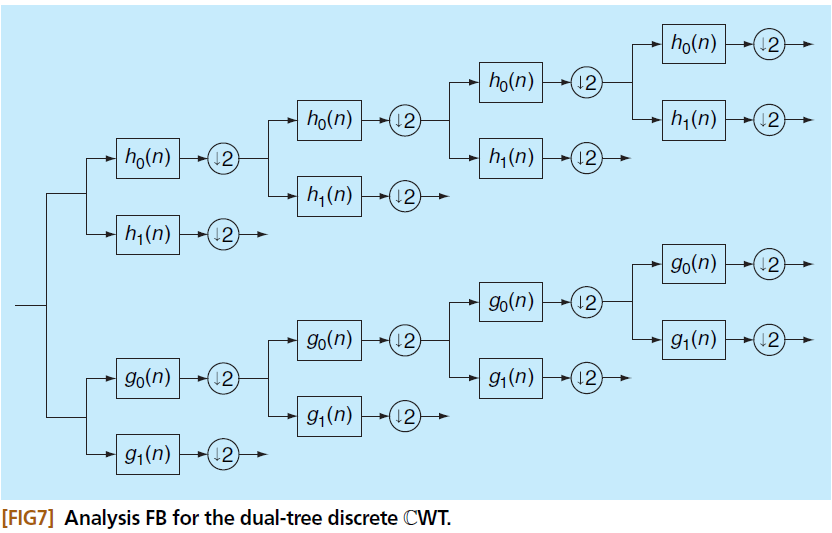
\includegraphics[width=\textwidth]{dt_analysis_fb}
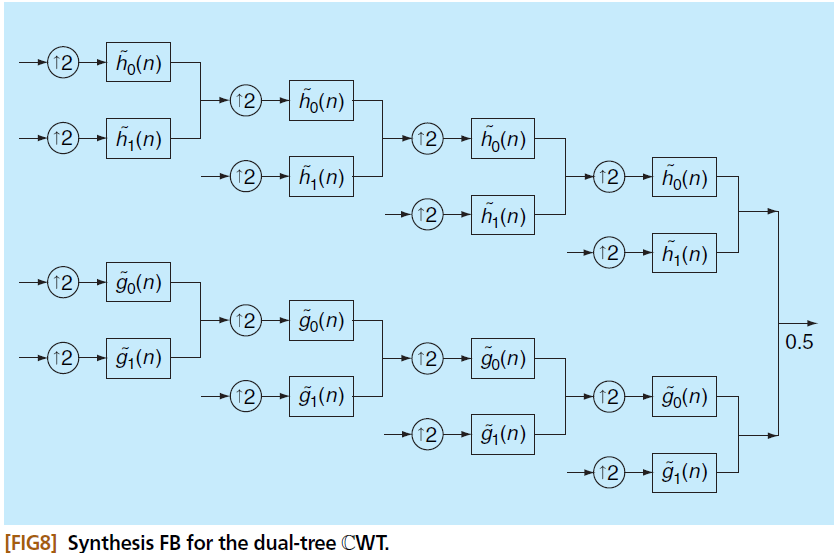
\includegraphics[width=\textwidth]{dt_synthesis_fb}
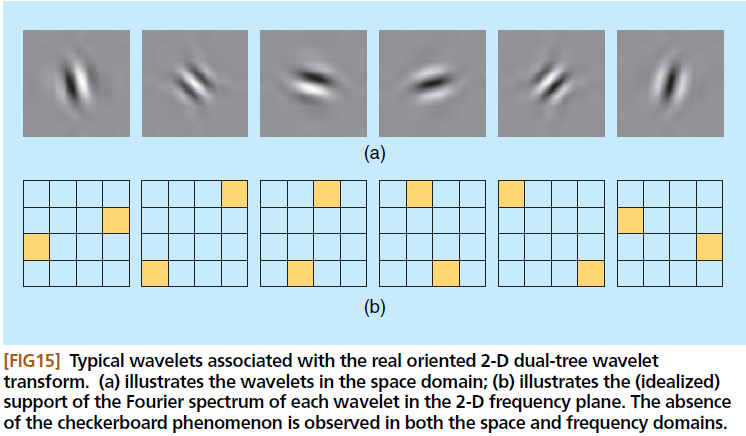
\includegraphics[width=\textwidth]{complex_dt_wav}
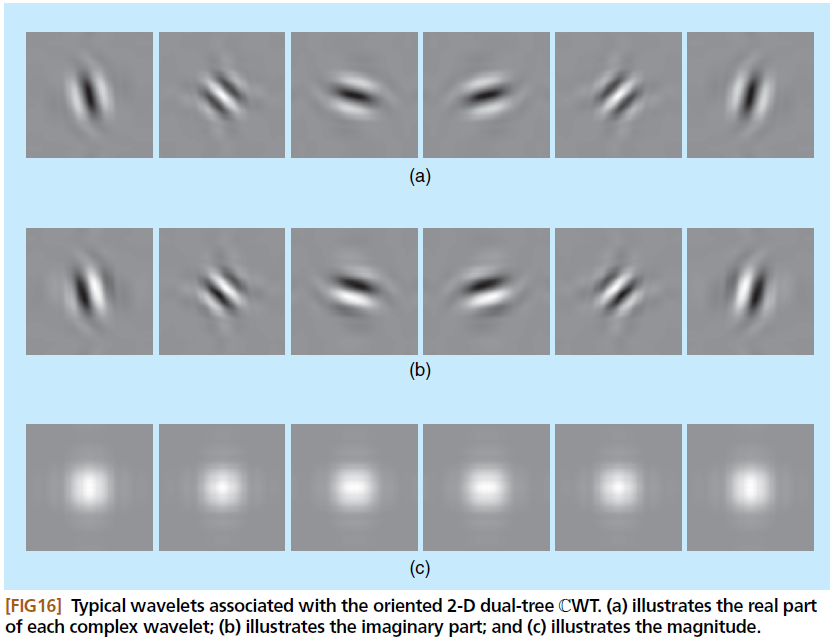
\includegraphics[width=\textwidth]{complex_oriented_wav}

\section{Sketching et $K$-means}
\subsection{$K$-means pour segmenter}
Ici on voit le problème d'un point de vue très statistique. On a pour données les (logs)-leaders $(l_{j,k})$, et par hypothèse, sur chaque texture\footnote{On désigne une texture par $t$, on peut se restreindre ici à $t\in \{0,1\}$, et on identifie les éléments de chaque texture à leur position multi-échelle.} $\{(j,k) \in \Omega_t\} = \Omega_t$, pour $t = 0,\cdots, K$ on a
\begin{equation}
	l_{j,k} \sim v_t + jh_t + \epsilon \iff (j,k)\in\Omega_t
\end{equation}
où $\epsilon$ est un bruit (gaussien pour faciliter les calculs et l'identification), qui pourrait dépendre de la texture $t$.
\par
On peut reformuler ce problème en $K$-means, avec $K=T$ le nombre de textures, donc on cherche $T$ paires de points $(v_t, h_t)_{t=1}^T$ qui minimisent
\begin{equation}
	\sum_{(j,k)} \min_{t=1,\cdots,T} || l_{j,k} - v_t - jh_t||.
\end{equation}
Une version alternative, pourrait être d'ignorer la relation d'échelle, et de chercher $TJ$  points $(s_{j,t})$ (où $J$ est le nombre d'échelles) en résolvant un $k$-means par échelle. L'avantage est qu'on a alors un problème $k$-means plus classique, et ensuite on peut faire une régression affine pour récupérer la relation d'échelle entre les coefficients\footnote{C'est peut être pas évident à faire parce que il faut réussir à mettre en correspondance les indices de textures $t$ entre les différentes échelles. Par contre je pense que c'est faisable dès que le nombre d'échelle est non négligeable $J>3$.}. Je pense qu'une reformulation un peu plus agréable de l'équation pourrait tout de même être faite.
\par
Une fois que l'on a obtenu les $T$-means, on a un moyen d'identifier chaque point à une texture, en définissant la segmentation $S: \{image\} \to \{textures\}$ par
\begin{equation}
	S : x = (J,k_x) \mapsto \hat{t}_x:= \arg\min_t ||l_{J,k_x} - v_t -Jh_t||
\end{equation}
ou une formule analogue (avec $k_x$ un indice de position aussi proche que possible de $x$ à l'échelle $J$). Je considère\footnote{Et c'est certainement ni vrai, ni optimal.} ici que l'information la plus fine est à l'échelle $J$ et c'est la plus précise. Une version pondérée à travers les échelles pourrait peut être donner de meilleurs résultats.

\subsection{Sketching}
Moralement on cherche à appliquer les idées du Compressed Sensing mais au lieu de faire des problèmes inverses sur des vecteurs, on le fait sur des distributions lineéaires.
\par
En compressed sensing, on a un opérateur linéaire de mesure $A$ (incohérent/aléatoire), que l'on applique à un signal (inconnu) $x$, qui nous donne une mesure $y$. Donc on a
\begin{equation}
	y = Ax
\end{equation} 
et on cherche à retrouver $x$. Sous des hypothèses de parcimonie (dans une base) de $x$, alors on peut reconstruire (si on connait la base) $x$. La reconstruction est garantie pour un problème compliqué (décomposition atomique), et à nouveau avec une hypothèse de parcimonie, le problème devient un problème pénalisé (en norme 1) qui est "facile".

\par
En sketching, on cherche à recontruire la distribution $\mathbb{P}_X$ d'une variable aléatoire $X$, et on se donne un opérateur $\mathcal{A}$ linéaire par rapport aux densités de probabilité\footnote{C'est à dire que pour deux variables aléatoires $X_1,X_2$ et $\alpha_1,\alpha_2$ des réels positifs et tels que $\alpha_1 + \alpha_2 = 1$, on peut définir la somme des densités de probabilité comme $d\mathbb{P} = \alpha_1d\mathbb{P}_{X_1} + \alpha_2d\mathbb{P}_{X_2}$ (qui est bien une densité de probabilité). Alors $\mathcal{A}$ est linéaire si pour toutes variables aléatoires et coefficients comme précédemment, on a 
$\mathcal{A}(d\mathbb{P}) = \mathcal{A}(\alpha_1d\mathbb{P}_1 + \alpha_2d\mathbb{P}_2) = \alpha_1\mathcal{A}(d\mathbb{P}_1) + \alpha_2\mathcal{A}(d\mathbb{P}_2)$. \newline

On peut remarquer que pour n'importe quelle fonction $f$, on a que $\mathbb{E}\circ f$ définit une application linéaire en ce sens.}. On mesure alors le sketch, idéalement,
\begin{equation}
	z = \mathcal{A}(X) = \mathbb{E}(\Phi(X))
\end{equation}
avec $\Phi$ une fonction de la variable aléatoire $X$.
 En pratique, on n'a pas accès à $X$, mais seulement à un échantillon $\mathcal{X} =\{x_1,\cdots, x_N\}$, et on définit donc
\begin{equation}
	\tilde z = \mathcal{A}(\mathcal{X}) = \frac{1}{N}\sum_{i=1}^N \Phi(x_i).
\end{equation}
L'intérêt est que l'on a
\begin{equation}
	\lim_{N\to\infty}\frac{1}{N}\sum_{i=1}^N\Phi(x_i) \to_{w.p.1} \mathcal{A}(X)
\end{equation} 
par la loi forte des grands nombres.
\newline
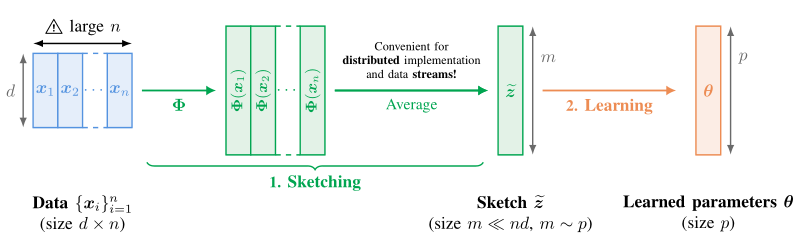
\includegraphics[width=\textwidth]{sketching_stream}
\par
Un avantage majeur, est que l'on est libre sur le choix de la fonction $\Phi$ et l'équation précédente reste vraie. Par exemple en prenant $\Phi: x\mapsto x^k$, $k\geq 0$, on a que le sketch de nos données converge vers le $k$-ième moment de la variable aléatoire (centrée) $X$. Pour cela, on peut parler de moment généralisé pour la fonction $\Phi$, ou le sketch, mais en fait on peut aller au delà des monomes.
\newline
Afin de retrouver quelle variable aléatoire a généré les données, on va chercher, parmi une classe de (densité de) variables aléatoires, la quelle a le sketch le plus proche du sketch des données, de type
\begin{equation}
	\arg\min_{d\mathbb{P}_X} || \Phi(\mathcal{X}) - \mathbb{E}_{d\mathbb{P}_X}(\Phi)||.
\end{equation}
 On peut par exemple faire de la PCA (linéaire) en prenant un moment généralisé $\Phi: x\mapsto x^Tx$, le sketch donne la matrice de covariance empirique. Afin de retrouver les composantes principales, il suffit de calculer la décomposition en valeurs singulière du sketch.
On peut aussi, avec d'autres $\Phi$ résoudre des problèmes type Least squares, Gaussian Mixture Modeling, $K$-means (cf références). Quelque chose d'important à remarquer est que le sketch ne donne généralement pas la solution du problème qui est en train d'être résolu. Mais par contre, une fois qu'on a un sketch de nos données, on peut calculer le problème inverse posé.
\newline
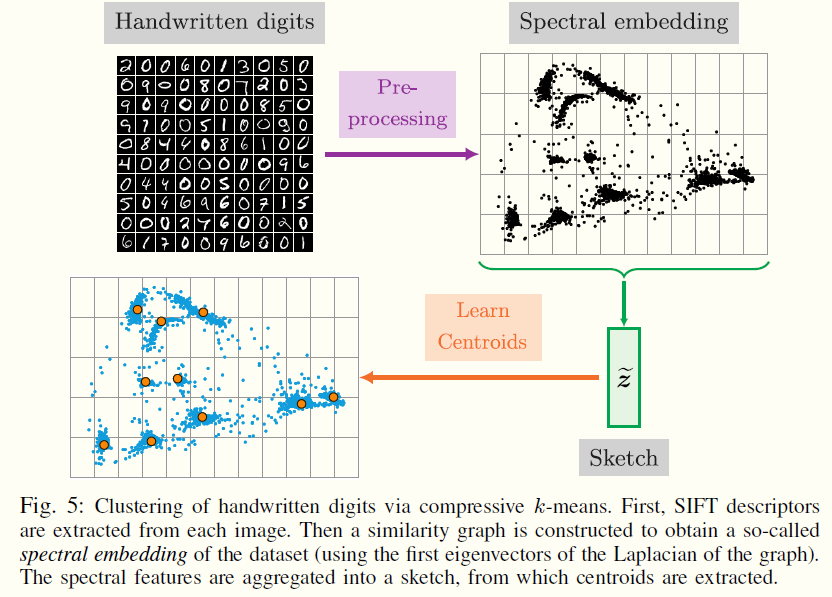
\includegraphics[width=\textwidth]{sketching_mnist}
\par
Un autre avantage est que la taille du sketch ne dépend pas du nombre de données à disposition. Ainsi, augmenter le nombre de données a seulement un coût pour calculer le sketch (ce qui est généralement très facile), mais par contre le coût de résolution du problème inverse reste constant (et devient même de mieux en mieux posé).
\newline
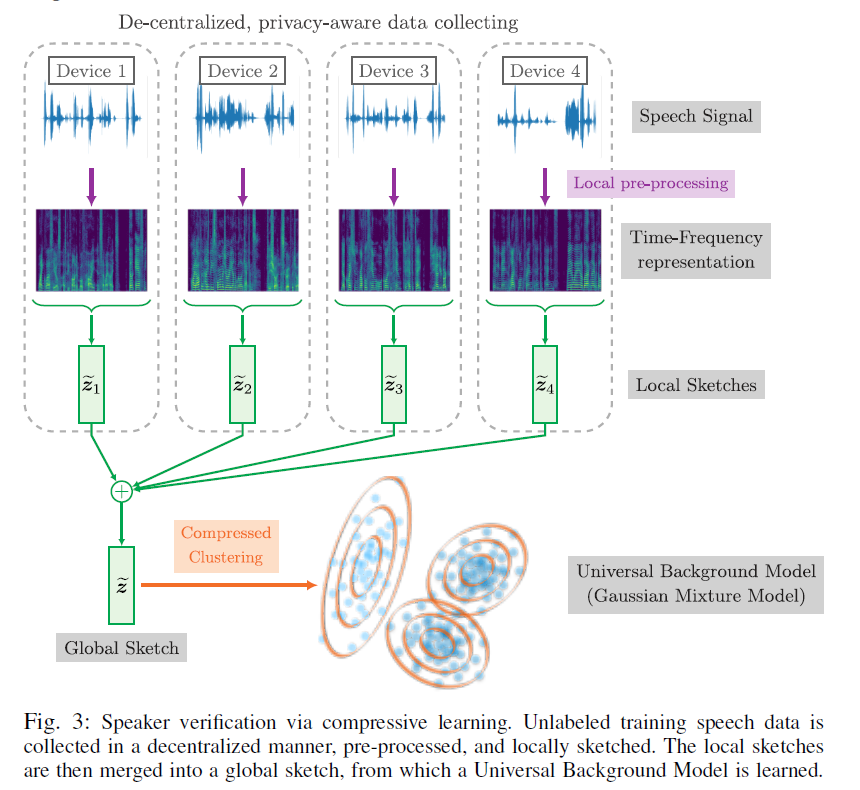
\includegraphics[width=\textwidth]{sketching_speak}
\par

Pour résoudre $K$-means, différents choix de sketch peuvent être utilisés, par exemple une binning map (qui correspond à un histogramme sur une partition de l'ensemble image de la variable aléatoire). Une autre alternative consiste à regarder les moments de Fourier aléatoire. En fait dans ce cadre, ça correspond juste à calculer la fonction génératrice de la distribution empirique, en passant à la limite on trouve bien avec proba 1 la fonction génératrice de la vraie distribution en tout point. On peut donc calculer le sketch en un certain nombre de fréquences, et ensuite on cherche à trouver une distribution qui a les mêmes valeurs en chaque fréquence afin de retrouver la distribution initiale. Ainsi, pour résoudre $K$-means, on cherche à trouver les $K$ (paires de) points $(v_t, h_t)$, qui minimisent
\begin{equation}\label{eq:prob1}
	||\tilde z - \sum_{t} \alpha_t \Phi(v_t, h_t)||
\end{equation} 
où les $\alpha_t$ sont tous positifs, et de somme égale  à 1. Moralement, $\alpha_t$ correspond au poids de la texture $t$ dans l'image d'origine, et $\Phi(v_t,h_t)$ correspond à la "signature" (une sorte d'échantillon spectral) d'une texture $t$. On verra plus bas comment expliciter un tel sketch.
\newline
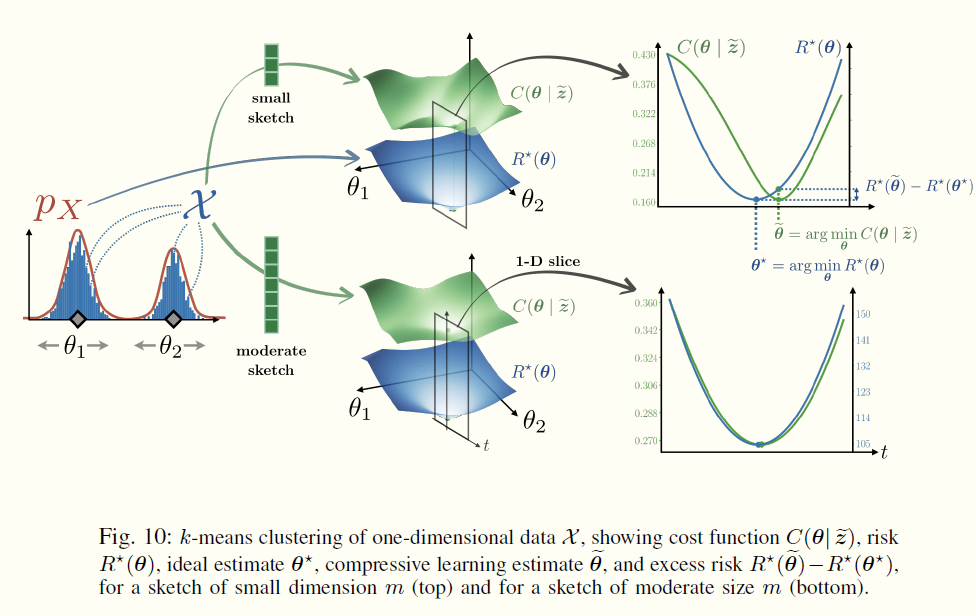
\includegraphics[width=\textwidth]{sketching_risk}

\subsection{Sketching, $K$-means et segmentation}
\par
On considère les logs-leaders $l = (l_j)_j = ((l_{j,k})_k)_j$ à travers les échelles et les positions (chacun de ces coefficients correspondant à un échantillon suivant une certaine loi). Dans un modèle $T$-means (sous reserve qu'il soit correct), à chaque échelle $j$, alors il existe $u_j \in \{\hat{l}_1,\cdots,\hat{l}_T\}^{N_j}$ qui minimise $||l_j - u||$, parmi tous les choix possibles de $u$ qui ne prennent que $T$ valeurs distinctes (avec $N_j$ le nombre total de coefficients de position à l'échelle $j$).
\par 
On peut par exemple considérer un sketch basé sur du Fourier aléatoire en prenant une suite de fréquence $\omega_1,\cdots, \omega_m$ (des nombres réels) et on pose
\begin{align}
	\Phi : \mathbb{R} &\to \mathbb{C}^m \\
		 x &\mapsto (e^{-i\omega_s x})_{s=1}^m.
\end{align}
Ce qui nous donne par exemple le sketch des logs-leaders à l'échelle $j$
\begin{equation}
	\tilde z_j = \frac{1}{N_j}\sum_{k=1}^{N_j} \Phi(l_{j,k}).
\end{equation}
En résumé
\begin{enumerate}
	\item On considère que chaque leader d'une image est un échantillon d'une variable aléatoire paramétrée uniquement par la texture à laquelle le point appartient, et qui vérifie une relation d'échelle 
	\item On a donc, à chaque échelle, $T$ distributions de probabilité que l'on cherche à estimer, et entre les échelles il existe une relation simple qui lie des distributions à travers les échelles
	\item On a donc accès à la distribution empirique des leaders, vue comme échantillon d'une somme de $T$-distributions
	\item On suppose que les $T$-means de notre distribution permettent d'identifier les textures
	\item On calcule le sketch pris sur toute l'image
	\item A partir du sketch on résoud un problème inverse pour retrouver les $T$-means (et possiblement leur relation inter-échelle)
\end{enumerate}

\subsubsection{Estimation échelle par échelle}
Pour l'instant on va considérer le problème à une échelle fixée, c'est à dire que l'on va d'abord chercher à estimer les centroides des logs-leaders de chaque texture et pas les coefficients de variance et régularité. Pour cela on peut chercher à trouver les $\alpha_t, \hat{l}_t$ (avec $\sum_t \alpha_t$ = 1) minimisant
\begin{equation}
	||\tilde z_j - \sum_t \alpha_t \Phi(\hat{l}_t)||.
\end{equation}
\par
Si on résoud ce problème à toutes les échelles, on obtient au final $J$ vecteurs de taille $T$ et afin d'identifier les textures, on peut dire que $J$ leaders représentent la même texture (chacun choisi à une échelle différente des autres parmi les leaders obtenus par $T$-means), si il existe une\footnote{En raison de la relation multi-échelle que l'on ne capture pas directement, plusieurs droites peuvent passer par un même point, par contre deux droites se croisent au plus une fois.(...)} droite qui passe parmi ces points. Cependant ce problème n'est peut-être pas tout à fait évident, on peut donc considérer le problème à travers les échelles directement.
\subsubsection{Estimation jointe à travers les échelles}

On va ici définir un sketch global à travers les échelles en utilisant la concatenation des sketchs $\tilde z_j$, ce qui nous donne 
\begin{align}
	\Phi_J : \mathbb{R}^J &\to \mathbb{C}^{Jm}\\
			(x_1,\cdots,x_J)&\mapsto (\Phi(x_1),\cdots, \Phi(x_J)).
\end{align}
On a donc le sketch correspondant $\tilde z = (\tilde z_1,\cdots, \tilde z_J)$. En utilisant l'hypothèse sur la relation d'échelle, on peut transformer le sketch global en un sketch qui ne dépend que de deux paramètres $(h,v)$:
\begin{align}
	\tilde \Phi :\mathbb{R}_+^2 &\to \mathbb{C}^{Jm}\\
			(h,v)&\mapsto \Phi_J(v + j_1h, v+j_2h,\cdots, v+Jh).
\end{align} 
On peut alors poser le problème d'optimisation sous la forme \ref{eq:prob1}. Commençons par expliciter $\tilde \Phi$ à une fréquence $\omega$, 
\begin{equation}
\tilde\Phi(h,v)(\omega) = (e^{-i\omega (v+j_1h)},\cdots, e^{-i\omega (v+Jh)}) = e^{-i\omega v}(e^{-i\omega j_1 h},\cdots, e^{-i\omega Jh})
\end{equation}
et ainsi le problème d'optimisation porte donc sur
\begin{equation}
	||(\frac{1}{N_1}\sum_{k} \Phi(l_{j_1, k}),\cdots, \frac{1}{N_J} \sum_k \Phi(l_{J,k})) - \sum_t \alpha_t \tilde\Phi(h_t,v_t) ||_{\mathbb{R}^{mJ}}
\end{equation}
où on minimise sur tous les $\alpha_t,h_t,v_t$ admissibles\footnote{Tous positifs, $h_t<1$ et $\sum_{t=1}^T \alpha_t = 1$.} et $m$ est le nombre de fréquences que l'on considère. Un problème équivalent est 
\begin{equation}
	\sum_{j} ||\frac{1}{N_j}\sum_{k} \Phi(l_{j, k}) - \sum_t \alpha_t \Phi( jh_t + v_t) ||_{\mathbb{R}^{m}}^2 = \sum_{j}^J \sum_{s}^m |\tilde z_{j}(\omega_s) - \sum_t \alpha_t e^{-i(v_t +jh_t)\omega_s}|^2
\end{equation}
où l'on minimise sur les mêmes paramètres.
\subsubsection{Segmentation}
Après résolution on a donc $(\alpha_t^*,h_t^*, v_t^*)_t$ qui minimise l'un des problèmes ci-dessus. Maintenant, il reste à faire la segmentation, c'est à dire assigner à un point (ou un leader) "ses" coefficients $h_t^*, v_t^*$. On peut penser à plusieurs méthodes, par exemple choisir la texture $t$ qui minimise l'erreur quadratique à travers les échelles entre la relation affine $v_t^* + jh_t^*$, ou bien la même chose à travers les sketch pris seulement dans un voisinage de la position considérée. C'est à dire,
\begin{equation}
	\hat{t}_x = \arg\min_t \sum_j (l_{j,k_{j,x}} - v_t^* - jh_t^*)^2
\end{equation}
ou bien
\begin{equation}
	\hat{t}_x = \arg\min_t ||\Phi_J(l_{j_1,k_{j_1,x}}, \cdots, l_{J,k_{J,x}} ) - \tilde\Phi(h_t^*,v_t^*)||_{\mathbb{R}^{Jm}}
\end{equation}
(je crois qu'il ne faut pas mettre le $\alpha_t^*$ ci-dessus).
\newline
Quelques références :
\begin{enumerate}
	\item Référence principale : \url{https://arxiv.org/abs/2008.01839}
	\item Résolution de $K$-means par sketching : \url{https://hal.inria.fr/hal-01386077v3/document}
	\item Quelques slides : \url{https://github.com/DavyL/sketching_slides/blob/main/main.pdf}
\end{enumerate}
\end{document}
